\documentclass[letter,10pt]{article}
\usepackage[utf8]{inputenc}
\usepackage[spanish, activeacute]{babel}
\usepackage{geometry}
\geometry{verbose,tmargin=0cm,bmargin=2cm,lmargin=2cm,rmargin=2cm,headheight=0cm,headsep=1cm,footskip=1cm}
\usepackage{graphicx}


%%%%%%%%%%%%%%%%%%%%%%%%%%%%%% Textclass specific LaTeX commands.
\newcommand{\lyxaddress}[1]{
\par {\raggedright #1
\vspace{1.4em}
\noindent\par}
}

%%%%%%%%%%%%%%%%%%%%%%%%%%%%%% User specified LaTeX commands.
\date{}

\begin{document}

\title{Problema F - ¿Y el problema F?}


\includegraphics[scale=0.6]{logo} \hspace*{9.00cm}

\includegraphics[scale=0.5]{dsc} 
\bigskip
\begin{center}
	\Large Problema F - ¿Y el problema F?
\end{center}

\begin{flushright}
Límite de tiempo: 3 segundos
\par\end{flushright}
\bigskip

\section*{Problema}

Se tiene una enorme cadena de caracteres la cual está codificada y tiene ciertas contraseñas escondidas, dependiendo del tipo y cantidad de contraseñas que contenga la cadena original se le asigna un valor, sabemos que podemos dividir dicha cadena en $N$ subcadenas que son propuestas como útiles, estas $N$ subcadenas pueden caer en uno de los siguientes 4 tipos de cadenas: cadenas palíndromos regulares, cadenas espejo, cadenas palíndromos espejo y cadenas basura, cada una de estas cadenas tiene un significado especial y un valor :

\begin{enumerate}
\item Palíndromos Regulares - Valor 1:

Cadena de caracteres que se lee igual hacia atras que hacia adelante. Ejemplo: ``RECONOCER''


\item Cadena Espejo - Valor 2:

Cadena de caracteres que, cuando se lee de atrás hacia adelante, cada caracter tiene su respectivo ``caracter espejo''. Ejemplo: ``3SI2E''.

Aquí se muestra la tabla de caracteres con sus correspondientes espejos, no todos los caracteres tiene un espejo.

\begin{figure}[h!]
  \begin{center}
  	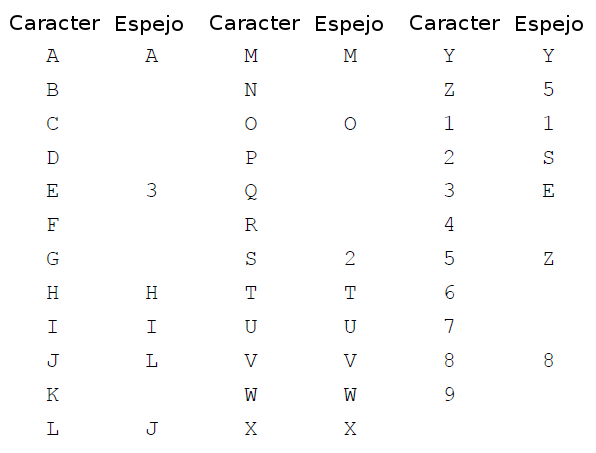
\includegraphics[scale=0.5]{adjunto}\caption{Tabla de caracteres}
  \end{center} 
\end{figure}

$$$$
$$$$
$$$$

\item Cadena Palíndromo Espejo - Valor 3:

Existen caracteres que son su mismo espejo, por ejemplo el espejo de ``A'' es ``A'' y el espejo de ``8'' es ``8'', una cadena palíndromo espejo es un palíndromo compuesto únicamente por caracteres que son su mismo espejo. Ejemplo: ``A8OMO8A''.


\item Cadena Basura - Valor 0:

Toda cadena que no cumple con alguna de las condiciones anteriores.
\end{enumerate}

Las cadenas palíndromo espejo tengan son las más especiales debido a que los investigadores están seguros de que son contraseñas de cuentas bancarias codificadas, sabiendo ésto, podemos obtener el valor de la cadena orginal, que es la suma de los valores de sus subcadenas.

Tu tarea es, dado un grupo de $M$ cadenas obtener cual es la que tiene mayor valor.

\subsection*{Entrada}

La primer línea de entrada será un número entero $N$, que indica el número de casos de prueba. Cada caso de prueba comienza con dos enteros $M$, ($1 \leq M \leq 10$) y $P$, ($1 \leq P \leq 50$), que indican el número de cadenas a evaluar y el número de subcadenas que contiene cada cadena, respectivamente. Cada cadena a evaluar está compuesta por dos lineas, la primera contiene la cadena y la segunda contiene $P$ enteros que son los índices donde termina cada subcadena, la subcadena 1 comienza en el índice 0. La longitud de cada cadena no sobrepasa los 10000 caracteres.

\subsection*{Salida}

Para cada caso de prueba debe de imprimirse: la cadena que tiene mayor valor, su número de cadenas espejo, la suma de los valores de sus subcadenas y sus subcadenas útiles ordenadas lexicográficamente, las cadenas basura no se consideran como cadenas útiles. Si existen varias cadenas con el mayor valor debe seleccionarse la que aparezca primero en la entrada.

\subsection*{Entrada ejemplo}
\noindent \texttt{1}~\\
\texttt{2 3}~\\
\texttt{NOTAPALINDROMEISAPALINILAPASIMIRRORED}~\\
\texttt{13 28 36}~\\
\texttt{2A3MEASATOYOTACOSAS}~\\
\texttt{6 13 18}~\\
\noindent 

\subsection*{Salida Ejemplo}

\noindent \texttt{2A3MEASATOYOTACOSAS}~\\
\texttt{1 5}~\\
\texttt{2A3MEAS}~\\
\texttt{ATOYOTA}~\\

\noindent \rule[0.5ex]{1\columnwidth}{1pt}


\lyxaddress{Mauricio Eduardo Montalvo Guzmán - Grupo de Algorimia Avanzada y Programación Competitiva}
\end{document}
